\title{rm_a2_concept}
\documentclass[12pt, a4paper]{report}
\usepackage[a4paper]{geometry}
\usepackage{lastpage}
\usepackage{graphicx, wrapfig, subcaption, setspace, booktabs}
\usepackage[T1]{fontenc}
\usepackage[font=small, labelfont=bf]{caption}
\usepackage{fourier}
\usepackage[protrusion=true, expansion=true]{microtype}
\usepackage[english]{babel}
\usepackage{sectsty}
\usepackage{hyperref}
\usepackage[table,xcdraw]{xcolor}

\onehalfspacing
\setcounter{tocdepth}{5}
\setcounter{secnumdepth}{5}

\usepackage[backend=biber,style=ieee,natbib=true]{biblatex}
\addbibresource{references.bib}

\begin{document}

\begin{titlepage}

\newcommand{\HRule}{\rule{\linewidth}{0.1mm}} % Defines a new command for the horizontal lines, change thickness here

\center % Center everything on the page

%----------------------------------------------------------------------------------------
%   MUK LOGO
%----------------------------------------------------------------------------------------

\begin{figure}
    \centering
  
\includegraphics[width=0.4\textwidth]{muklogo.png}
\end{figure}
 
%----------------------------------------------------------------------------------------
%   HEADING SECTIONS
%----------------------------------------------------------------------------------------

\textsc{\LARGE Makerere University}\\[0.7cm] % Name of your university/college
\textsc{\Large CoCIS / SoCIT}\\[0.2cm] % Major heading such as course name
\textsc{\large B.Sc. Computer Science}\\[0.1cm] % Minor heading such as course title
\textsc{\small BIT 2207 Research Methodology}\\[0.8cm]

%----------------------------------------------------------------------------------------
%   TITLE SECTION
%----------------------------------------------------------------------------------------

\HRule \\[0.6cm]
\textsc{\Large Detecting structure in voters' preferences}\\[0.4cm]
\small{\textsc{A concept paper}}
\HRule \\[1.0cm]
 
%----------------------------------------------------------------------------------------
%   AUTHOR SECTION
%----------------------------------------------------------------------------------------

% \begin{minipage}{0.4\textwidth}
% \begin{flushleft} \large
% \emph{Author:}\\
% John \textsc{Smith} % Your name
% \end{flushleft}
% \end{minipage}
% ~
% \begin{minipage}{0.4\textwidth}
% \begin{flushright} \large
% \end{flushright}
% \end{minipage}\\[4cm]

% \large
% PETER \textsc{Rutabingwa}\\
% \textsc{15/U/12443/EVE}\\[3cm] % Your name

\begin{table}[!hb]
\centering
\begin{tabular}{|l|l|l|}
\hline
Abdul \textsc{Kizza Ntale} & \textsc{15/U/11561/EVE} \\ \hline
Harold \textsc{Turyasingura} & \textsc{10/U/11447/EVE} \\ \hline
Peter \textsc{Rutabingwa} & \textsc{15/U/12443/EVE} \\ \hline
Williams \textsc{kakooza} & \textsc{15/U/20165/EVE} \\
\hline
\end{tabular}
\end{table}

{\large April 21, 2017}

\vfill

\end{titlepage}

\tableofcontents
\newpage

\sectionfont{\scshape}
%----------------------------------------------------------------------------------------
%   SECTION
%----------------------------------------------------------------------------------------
\section*{Introduction}
\addcontentsline{toc}{section}{Introduction}
Structured preference domains, such as, for example, the domains of single-peaked and single-crossing preferences, are known 

to admit efficient algorithms for many problems in computational social choice. Some of these algorithms extend to 

preferences that are close to having the respective structural property, i.e., can be made to enjoy this property by performing 

minor changes to voters’ preferences, such as deleting a small number of voters or candidates. However, it has recently been 

shown that finding the optimal number of voters or candidates to delete in order to achieve the desired structural property is 

NP-hard for many such domains. In this paper, we show that these problems admit efficient approximation algorithms. Our 

results apply to all domains that can be characterized in terms of forbidden configurations; this includes, in particular, single-

peaked and single-crossing elections. For a large range of scenarios, our approximation results are optimal under a plausible 

complexity-theoretic assumption. We also provide parameterized complexity results for this class of problems.

\subsection*{Background}
\addcontentsline{toc}{subsection}{Background}
 Collective decision-making plays an important role in the functioning of multi-agent systems or people. Typically, it is assumed 

that agents are given a set of alternatives (sometimes also called the candidates), and need to select a non-empty subset of this 

set; each agent’s preferences over the candidates are usually represented by a total order over the candidate set. Making a 

collectively optimal choice in this setting is often a difficult problem, as evidenced by Arrow’s classic impossibility result (1951). 

Therefore, collective decision making is often studied under the assumption that agents’ preferences satisfy additional 

constraints. Perhaps the most famous example of a restricted preference domain is the domain of single-peaked preferences 

(Black 1958); other examples include single-caved preferences (Inada 1964), single-crossing preferences (Mirrlees 1971), value-

restricted preferences (Sen 1966), and group separable preferences (Inada 1964; 1969). Many of these domains enjoy desirable 

social choice-theoretic properties, such as transitivity of the majority relation and existence of a strategy proof social choice 

rule (Barbera and Moreno2011). Moreover, it has recently been shown that many hard algorithmic problems pertaining to voting 

and elections become easier if the voters’ preferences can be assumed to be single-peaked or single-crossing (Faliszewski et al. 

2011; Brandt et al. 2010; Cornaz, Galand, and Spanjaard 2012; 2013; Skowron et al. 2013); it seems plausible that some of these 

results could be extended to other restricted domains. Further, some of these efficient algorithms can be modified to work for 

preference profiles that are close to being single-peaked or single-crossing, for an appropriate notion of closeness (Faliszewski, 

Hemaspaandra, and Hemaspaandra 2014; Cornaz, Galand, and Spanjaard 2012; 2013; Yang and Guo 2014a; 2014b).
\subsection*{Problem Statement}
\addcontentsline{toc}{subsection}{Problem Statement}

 Now, suppose that we have a polynomial-time algorithm for some voting-related problem on a restricted domain D. To use this 

algorithm, we may have to be able to detect whether a given election belongs to D. For commonly studied domains, such as 

single-peaked and single-crossing preferences this can be done efficiently (Bartholdi and Trick 1986; Escoffier, Lang, and Ozt ¨ 

urk 2008; Bredereck, Chen, ¨ and Woeginger 2013b; Elkind, Faliszewski, and Slinko 2012). However, it has recently been shown 

that determining if an election is close to being in a restricted domain is computationally difficult, for many such domains and 

many notions of closeness. More specifically, Erdelyi et al. (2013) focus on the single-peaked domain, and investigate the 

complexity of computing the “distance” between a given election and this domain. They consider a variety of distance measures, 

such as the number of voters or candidates that need to be deleted or the number of candidate swaps that need to be performed 

to make the election single-peaked, as well as distances that are based on splitting voters or candidates into several groups. In 

particular, Erdelyi et al. show that finding a minimum-size set of voters to delete in order to make an election single-peaked is 

NP-hard; in contrast, for candidate deletion this problem is in P. A related paper by Bredereck et al. (2013a) only considers two 

distance measures, namely, the candidate deletion distance and the voter deletion distance, but explores several restricted 

preference domains, including single-caved and single-crossing preferences, best-/worst-/medium-/value-restricted 

preferences and group-separable preferences. It shows that many of the associated computational problems are NP-hard; an 

important exception is the problem of finding a minimum-size set of voters whose deletion results in a single-crossing election, 

which admits a polynomial-time algorithm. These NPhardness results present a difficulty if one wants to use efficient algorithms 

for nearly structured domains, as some of these algorithms rely on knowing the “distance” to the respective domain. It is then 

natural to ask if these hardness results can be circumvented using approximation algorithms and/or parameterized algorithms. 

The main contribution of our paper is answering this question in the affirmative for the voter deletion distance and the 

candidate deletion distance, and for a large family of restricted domains. Specifically, our results apply to any restricted domain 

that can be characterized in terms of forbidden configurations (see Section 2); this includes all domains discussed by Bredereck 

et al. (2013a). We demonstrate that for any such domain D the problem of finding the smallest number of voters/candidates to 

delete in order to obtain an election in D admits an efficient approximation algorithm. To do so, we reduce our problem to the 

classic HITTING SET problem. The approximation ratio on our algorithm is determined by the size of the largest forbidden 

configuration used to characterize D, which is typically a small integer. For the voter deletion distance and several restricted 

domains (including, notably, the single-peaked domain), we can improve the approximation ratio of our algorithm by using a 

more elaborate reduction to HITTING SET; this approach results in a 2-approximation algorithm. We show that this result is 

optimal subject to the Unique Games Conjecture (Khot and Regev 2008), which is a wellknown complexity-theoretic 

assumption. Our reduction to HITTING SET also allows us to use parameterized algorithms for this problem, resulting in FPT 

algorithms for our problem. For a summary of approximation and FPT results, we refer to Table 1. For voter deletion, we also 

consider the setting where we need to delete more than half of the voters. In this case, it is more natural to focus on computing 

the number of surviving voters. We show that this problem is W[1]-complete, and cannot be approximated within n 1−unless P 6= 

NP. We omit some proofs due to space constraints.
\subsection*{Aim and Objectives}
\addcontentsline{toc}{subsection}{Aim and Objectives}
Given a positive integer s, we write [s] to denote the set {1, . . . , s}. When discussing fixed-parameter algorithms, we use the 

standard notation of parameterized complexity, and write O∗ (f(k)) as a shorthand for O(f(k)• n O(1)), i.e., the O∗ notation 

ignores polynomial factors. Elections and restricted preference domains. An election is described by a set of candidates C = {c1, . 

. . , cm} and a list of votes V = (v1, . . . , vn), where each vi , i ∈ [n], is a complete order over C; we refer to vi as the vote, or 

preferences, of voter i, and write E = (C, V ). The list of votes V is sometimes called the preference profile. If vi ranks candidate a 

above candidate b, we write a >i b or vi : ab. Given a list of votes V 0 , we write V 0 ⊆ V if V 0 can be obtained from V by deleting 

some of the votes; further, given V 0 ⊆ V , we write V \ V 0 to denote the list of votes that can be obtained from V by removing 

the votes in V 0 .
In what follows, we discuss restricted preference domains, i.e., sets of elections that satisfy certain properties. The most 

prominent examples of such domains are single-peaked preferences and single-crossing preferences. Definition 1. A vote vi 

over a candidate set C is said to be single-peaked with respect to a complete order ¬ over C if for every triple of candidates a, b, c 

∈ C such that a ¬ b ¬ c or c ¬ b ¬ a it holds that a >i b implies b >i c. An election E = (C, V ) is said to be single-peaked if there 

exists a complete order ¬ over C such that every vote in V is single-peaked with respect to ¬. Definition 2. An election E = (C, V ), 

where V = (v1, . . . , vn), is said to be single-crossing with respect to V if for every pair of candidates a, b ∈ C such that a >1 b all 

voters in V that rank a above b precede all voters in V that rank b above a. Further, E = (C, V ) is said to be single-crossing if the 

votes in V can be permuted so that E is single-crossing with respect to the resulting ordering V 0 . Our results apply to several 

other restricted preference domains, including worst-/best-/medium-/value-restricted, single-caved and group-separable 

preferences. We define the first four of these domains in Section 3. The remaining definitions are omitted, as they are not 

essential for our presentation; see, e.g., (Bredereck, Chen, and Woeginger 2013a).

Configurations A condition on a set of variables X = {x1, . . . , xt} is a Boolean formula with pairwise comparisons of x1, . . . , xt as 

atoms. For instance, φ : x1 > x2 ∧ x3 > x4 (or short: φ : x1x2 ∧ x3x4) is a condition on {x1, x2, x3, x4}. Let ||φ|| denote the 

description size of a condition. Since we only consider conditions over domains of small constant size, the representation details 

do not affect the complexity of our algorithms. A configuration is a set of conditions Φ = {φ1, . . . , φs}, where all φi , i ∈ [s], are 

conditions over the same set of variables. We denote by s(Φ) the number of conditions in Φ and by X(Φ) the set of variables that 

occur in Φ; also, we write t(Φ) = |X(Φ)|. We refer to a configuration Φ with s(Φ) = s, t(Φ) = t as an (s, t)-configuration. The 

following definition plays a central role in this paper. Definition 3. Given a mapping ξ : X → C and a condition φ over X, let ξ(φ) 

denote the Boolean formula obtained by replacing all variables in φ according to ξ. We say that a vote v over C fulfills φ with 

respect to ξ (and write v |=ξ φ) if v is a model for ξ(φ). An election E = (C, V ) is said to contain a configuration Φ = {φ1, . . . , φs} 

with X(Φ) = X if there exists a mapping ξ : X → C and s distinct votes vi1 , . . . , vis ∈ V such that vij |=ξ φj for all j ∈ [s]. Example 1. 

Consider an election E = (C, V ), where C = {c1, c2, c3, c4}, V = (v1, v2), v1 : c1c2c3c4, v2 : c4c1c2c3, and a configuration Φ = {φ1, φ2}, 

where φ1 : abc, φ2 : bca. Then E contains Φ. Indeed, if we set ξ(a) = c4, ξ(b) = c1, ξ(c) = c2, vi1 = v2, vi2 = v1, we get vi1 |=ξ φ1, vi2 |=ξ 

φ2. We will now introduce five configurations that will play an important role in this paper.  
\begin{figure}
    \centering
  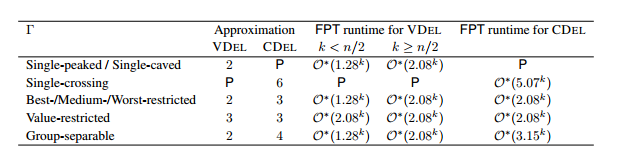
\includegraphics[width=0.4\textwidth]{configurations.png}
\end{figure}



\subsubsection*{Aim}
\addcontentsline{toc}{subsubsection}{Aim}
 The α-configuration is a (2, 4)-configuration Φα with conditions φ1 : abc ∧ db, φ2 : cba ∧ db. The worst-diverse configuration is a 

(3, 3)-configuration ΦW with conditions φ1 : ac ∧ bc, φ2 : ab ∧ cb, φ3 : ba ∧ ca. The best-diverse configuration is a (3, 3)-

configuration ΦB with conditions φ1 : ab ∧ ac, φ2 : ba ∧ bc, φ3 : ca ∧ cb. The medium-diverse configuration is a (3, 3)-

configuration ΦM with conditions φ1 : bac ∨ cab, φ2 : abc ∨ cba, φ3 : acb ∨ bca. The value-diverse configuration is a (3, 3)-

configuration ΦC with conditions φ1 : abc, φ2 : bca, φ3 : cab. An election is said to be worst-restricted if it contains no 

occurrences of ΦW ; best-restricted, medium-restricted, and value-restricted elections are defined similarly. We will now 

formulate two simple conditions on configurations. Definition 5. A configuration Φ is exact if every preference order over X(Φ) 

fulfills at most one condition in Φ. Further, Φ is partitioning if every preference order over X(Φ) fulfills exactly one condition in 

Φ. Observe that Φα, ΦW , ΦB , ΦM , and ΦC are exact con- figurations; further, ΦW , ΦB , and ΦM are partitioning, but Φα and 

ΦC are not. The notion of partitioning configuration will play an important role in Section 5. We will now describe an efficient 

algorithm for checking whether an election E contains an exact configuration Φ. Proposition 6. Given an exact configuration Φ 

with s(Φ) = s, t(Φ) = t and an election E = (C, V ) with |C| = m, |V | = n, we can detect whether E contains Φ in time O(||Φ|| nmt ). 

Proof. We can go over all ordered t-tuples of elements of C. Each such tuple can be interpreted as a mapping ξ from X = X(Φ) to 

C. For each such mapping, we set Φ 0 = Φ and go over the votes in V one by one. For each vote v ∈ V , we check whether v |=ξ φi 

for some φi ∈ Φ 0 ; this can be done in time O(||Φ||). Note that, since Φ is exact, there can be at most one such condition. If v |=ξ 

φi , we remove φi from Φ 0 , and repeat this process with the next vote in V . 
\subsubsection*{Specific Objectives}
\addcontentsline{toc}{subsubsection}{Specific Objectives}
If Φ 0 becomes empty, we return “yes” and stop. If all votes in V have been processed, but Φ 0 remains non-empty, we move on 

to the next mapping ξ : X → C (and reset Φ 0 = Φ). If we have enumerated all mappings ξ : X → C, we stop and output “no”. The 

correctness of this algorithm and the bound on its running time are immediate. If Φ is not exact, the algorithm described in the 

proof of Proposition 6 may fail to work correctly. However, by considering all mappings ξ : X → C and all ordered s-tuples of 

voters in V , we can check whether E contains Φ in time O(||Φ|| n smt ). We say that a preference domain D is characterized by a 

set of forbidden configurations Γ = {Φ1, . . . , Φγ} if for every election E we have E ∈ D if and only if E does not contain any of the 

configurations in Γ. By definition, the domains of worst-restricted, bestrestricted, medium-restricted, and value-restricted 

elections can be characterized by sets of forbidden configurations that consist of a single (3, 3)-configuration each. Moreover, 

the following results are known. • The domain of single-peaked preferences is characterized by the set of forbidden 

configurations {Φα, ΦW } (Ballester and Haeringer 2011). • The domain of single-crossing preferences is characterized by a set of 

forbidden configurations {Φγ, Φδ}, where Φγ is a (3, 6)-configuration and Φδ is a (4, 4)-configuration (Bredereck, Chen, and 

Woeginger 2013b). • The domain of single-caved preferences is characterized by a set of forbidden configurations {Φα¯, ΦB }, 

where Φα¯ is a (2, 4)-configuration (Ballester and Haeringer 2011). • The domain of group-separable preferences is characterized 

by a set of forbidden configurations {Φβ, ΦM }, where Φβ is a (2, 4)-configuration (Ballester and Haeringer 2011). Each of the 

configurations Φα¯, Φβ, Φγ, Φδ is exact. We set ΓW = {ΦW }, ΓB = {ΦB }, ΓM = {ΦM }, ΓC = {ΦC }, Γsp = {Φα, ΦW }, Γscv = {Φα¯, ΦB 

}, Γsc = {Φγ, Φδ}, Γgs = {Φβ, ΦM }. We will now define the two families of computational problems that will be the focus of this 

paper. Both families are parameterized by a set of configurations Γ.
\begin{figure}[ht!]
\centering
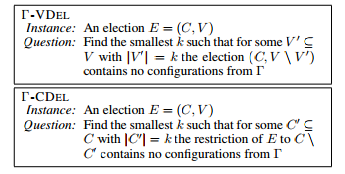
\includegraphics[width=90mm]{instance.png}
\caption{Families \label{overflow}}

\end{figure}

\subsection*{Significance}
\addcontentsline{toc}{subsection}{Significance}
A Simple Conversion to Hitting Set
In this section, we describe a straightforward transformation from Γ-VDEL and Γ-CDEL to the classic HITTING SET problem. We 

start by defining this problem formally. 
\begin{figure}[ht!]
\centering
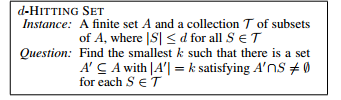
\includegraphics[width=90mm]{setprob.png}
\caption{Problem set \label{overflow}}
\addcontentsline{toc}{subsection}{Significance}
Let Γ be a set of exact configurations, let ||Γ|| = P Φ∈Γ ||Φ||, and let s = maxΦ∈Γ s(Φ), t = maxΦ∈Γ t(Φ). Then an instance E = (C, 

V ) of Γ-VDEL (respectively, Γ-CDEL) with |C| = m, |V | = n can be reduced to an instance (A, T ) of d-HITTING SET with d = s 

(respectively, d = t) in time O(||Γ|| nmt ) so that the optimal number of voters (respectively, candidates) to delete in E equals the 

optimal size of the hitting set for (A, T ). Proof. We first consider Γ-VDEL. Given an election E = (C, V ), we set A = V . Further, for 

each occurrence of a forbidden configuration from Γ in E we add the corresponding set of voters to T . We obtain an instance of 

d-HITTING SET with d = maxΦ∈Γ s(Φ). For Γ-CDEL, the reduction is similar: we set A = C, and the sets in T correspond to sets of 

candidates in occurrences of configurations from Γ in E. Let (A, T ) be the instance of d-HITTING SET produced by our 

reduction. Suppose that we can eliminate all occurrences of the configurations in Γ from E by deleting a set of voters V 0 ⊆ V . 

Then V 0 intersects every set in T , so (A, T ) admits a hitting set of size |V 0 |. Conversely, if A0 is a hitting set for (A, T ), then by 

deleting the corresponding voters from V we ensure that our election contains no configurations in Γ. A similar argument works 

for Γ-CDEL. To implement this reduction, we go over all configurations in Γ, and, for each configuration Φ, detect all 

occurrences of Φ in E using a modification of the algorithm described in Proposition 6. This establishes the bound on the 

running time of our reduction. This simple conversion enables us to use the techniques developed for d-HITTING SET in order 

to solve Γ-VDEL and Γ-CDEL whenever all configurations in Γ are exact and t = maxΦ∈Γ t(Φ) is bounded by a small constant; this 

is the case for all sets of forbidden configurations considered in this paper. These techniques include, in particular, 

approximation algorithms and FPT algorithms for d-HITTING SET. However, the running time and/or solution quality of these 

algorithms often depends on the value of d. Thus, it would be desirable to have a reduction that produces an instance of d-

HITTING SET with a smaller value of d. We will now see that this is indeed possible for Γ-VDEL, for several important sets of 

forbidden configurations Γ, including the one that characterizes single-peaked preferences. 5 An Improved Conversion to 

Hitting Set Our improved conversion from Γ-VDEL to d-HITTING SET relies on the notion of a partitioning configuration 

(Definition 5). Given an election E = (C, V ) and a mapping ξ : X → C, a partitioning (s, t)-configuration Φ = {φ1, . . . , φs} with X(Φ) 

= X induces a partition of V into s sets V ξ 1 , . . . , V ξ s , where V ξ i = {v ∈ V | v |=ξ φi} for each i ∈ [s]. Using this observation, for 

Γ-VDEL we can strengthen Theorem 7 as follows. Theorem 8. Let Γ be a set of exact configurations, let ||Γ|| = P Φ∈Γ ||Φ||, and let 

s = maxΦ∈Γ s(Φ), t = maxΦ∈Γ t(Φ), where s ≥ 3. Suppose also that Γ contains exactly one configuration Φ + with s(Φ+) = s, and 

this configuration is partitioning. Then, given an instance E = (C, V ) of Γ-VDEL with |C| = m, |V | = n, where the optimal solution 

size is less than n s−1 , we can construct s instances of (s − 1)-HITTING SET in time O(||Γ|| nmt ) so that the optimal number of 

voters to delete in E equals mini∈[s] |Ai |, where Ai is an optimal hitting set for the i-th instance. Proof. We construct s instances 

of (s − 1)-HITTING SET, denoted by (A, T1),(A, T2), . . . ,(A, Ts). We set A = V . The sets T1, . . . , Ts are constructed in three steps. 

Step 1. Let Φ + = {φ1, . . . , φs} be the unique configuration in Γ with s(Φ+) = s; let X = X(Φ+). As explained above, for every 

mapping ξ : X → C, Φ + defines a partition of V into sets of votes V ξ 1 , . . . , V ξ s . Pick a mapping ξ that maximizes the size of the 

smallest set in {V ξ 1 , . . . , V ξ s }. For each i ∈ [s], initialize Ti by setting Ti = {{v} | v ∈ V ξ i }. Step 2. Let V−i = V \ V ξ i for all i ∈ [s]. 

We will now iterate over all mappings ξ 0 : X → C and for every such mapping we consider its induced partition of V−i . We denote 

the sets in this partition by V ξ 0 ,i 1 , . . . , V ξ 0 ,i s and assume without loss of generality that |V ξ 0 ,i 1 | ≤ . . . ≤ |V ξ 0 ,i s |. For 

each tuple (vi1 , . . . , vis−1 ) ∈ V ξ 0 ,i 1 × • • • × V ξ 0 ,i s−1 we add the set {vi1 , . . . , vis−1 } to Ti . Step 3. It remains to deal with 

configurations in Γ \ {Φ +}; by our assumption, we have s(Φ) ≤ s − 1 for every Φ ∈ Γ\{Φ +}. We handle them in the same way as in 

Theorem 7, i.e., for each i ∈ [s] and each Φ 0 ∈ Γ \ {Φ} we add to Ti all sets of voters that correspond to occurrences of Φ 0 in E. 

This completes the description of our reduction. The bound on its running time is immediate. Also, each Ti , i ∈ [s], only 

contains sets of size s − 1 or less, i.e., we have constructed s instances of (s − 1)-HITTING SET. 

\section*{Methodology}
\addcontentsline{toc}{section}{Methodology}
Theorem 7. Let Γ be a set of exact configurations, let ||Γ|| = P Φ∈Γ ||Φ||, and let s = maxΦ∈Γ s(Φ), t = maxΦ∈Γ t(Φ). Then an 

instance E = (C, V ) of Γ-VDEL (respectively, Γ-CDEL) with |C| = m, |V | = n can be reduced to an instance (A, T ) of d-HITTING SET 

with d = s (respectively, d = t) in time O(||Γ|| nmt ) so that the optimal number of voters (respectively, candidates) to delete in E 

equals the optimal size of the hitting set for (A, T ). Proof. We first consider Γ-VDEL. Given an election E = (C, V ), we set A = V . 

Further, for each occurrence of a forbidden configuration from Γ in E we add the corresponding set of voters to T . We obtain an 

instance of d-HITTING SET with d = maxΦ∈Γ s(Φ). For Γ-CDEL, the reduction is similar: we set A = C, and the sets in T correspond 

to sets of candidates in occurrences of configurations from Γ in E. Let (A, T ) be the instance of d-HITTING SET produced by our 

reduction. Suppose that we can eliminate all occurrences of the configurations in Γ from E by deleting a set of voters V 0 ⊆ V . 

Then V 0 intersects every set in T , so (A, T ) admits a hitting set of size |V 0 |. Conversely, if A0 is a hitting set for (A, T ), then by 

deleting the corresponding voters from V we ensure that our election contains no configurations in Γ. A similar argument works 

for Γ-CDEL. To implement this reduction, we go over all configurations in Γ, and, for each configuration Φ, detect all 

occurrences of Φ in E using a modification of the algorithm described in Proposition 6. This establishes the bound on the 

running time of our reduction. This simple conversion enables us to use the techniques developed for d-HITTING SET in order 

to solve Γ-VDEL and Γ-CDEL whenever all configurations in Γ are exact and t = maxΦ∈Γ t(Φ) is bounded by a small constant; this 

is the case for all sets of forbidden configurations considered in this paper. These techniques include, in particular, 

approximation algorithms and FPT algorithms for d-HITTING SET. However, the running time and/or solution quality of these 

algorithms often depends on the value of d. Thus, it would be desirable to have a reduction that produces an instance of d-

HITTING SET with a smaller value of d. We will now see that this is indeed possible for Γ-VDEL, for several important sets of 

forbidden configurations Γ, including the one that characterizes single-peaked preferences. 5 An Improved Conversion to 

Hitting Set Our improved conversion from Γ-VDEL to d-HITTING SET relies on the notion of a partitioning configuration 

(Definition 5). Given an election E = (C, V ) and a mapping ξ : X → C, a partitioning (s, t)-configuration Φ = {φ1, . . . , φs} with X(Φ) 

= X induces a partition of V into s sets V ξ 1 , . . . , V ξ s , where V ξ i = {v ∈ V | v |=ξ φi} for each i ∈ [s]. Using this observation, for 

Γ-VDEL we can strengthen Theorem 7 as follows. Theorem 8. Let Γ be a set of exact configurations, let ||Γ|| = P Φ∈Γ ||Φ||, and let 

s = maxΦ∈Γ s(Φ), t = maxΦ∈Γ t(Φ), where s ≥ 3. Suppose also that Γ contains exactly one configuration Φ + with s(Φ+) = s, and 

this configuration is partitioning. Then, given an instance E = (C, V ) of Γ-VDEL with |C| = m, |V | = n, where the optimal solution 

size is less than n s−1 , we can construct s instances of (s − 1)-HITTING SET in time O(||Γ|| nmt ) so that the optimal number of 

voters to delete in E equals mini∈[s] |Ai |, where Ai is an optimal hitting set for the i-th instance. Proof. We construct s instances 

of (s − 1)-HITTING SET, denoted by (A, T1),(A, T2), . . . ,(A, Ts). We set A = V . The sets T1, . . . , Ts are constructed in three steps. 

Step 1. Let Φ + = {φ1, . . . , φs} be the unique configuration in Γ with s(Φ+) = s; let X = X(Φ+). As explained above, for every 

mapping ξ : X → C, Φ + defines a partition of V into sets of votes V ξ 1 , . . . , V ξ s . Pick a mapping ξ that maximizes the size of the 

smallest set in {V ξ 1 , . . . , V ξ s }. For each i ∈ [s], initialize Ti by setting Ti = {{v} | v ∈ V ξ i }. Step 2. Let V−i = V \ V ξ i for all i ∈ [s]. 

We will now iterate over all mappings ξ 0 : X → C and for every such mapping we consider its induced partition of V−i . We denote 

the sets in this partition by V ξ 0 ,i 1 , . . . , V ξ 0 ,i s and assume without loss of generality that |V ξ 0 ,i 1 | ≤ . . . ≤ |V ξ 0 ,i s |. For 

each tuple (vi1 , . . . , vis−1 ) ∈ V ξ 0 ,i 1 × • • • × V ξ 0 ,i s−1 we add the set {vi1 , . . . , vis−1 } to Ti . Step 3. It remains to deal with 

configurations in Γ \ {Φ +}; by our assumption, we have s(Φ) ≤ s − 1 for every Φ ∈ Γ\{Φ +}. We handle them in the same way as in 

Theorem 7, i.e., for each i ∈ [s] and each Φ 0 ∈ Γ \ {Φ} we add to Ti all sets of voters that correspond to occurrences of Φ 0 in E. 

This completes the description of our reduction. The bound on its running time is immediate. Also, each Ti , i ∈ [s], only 

contains sets of size s − 1 or less, i.e., we have constructed s instances of (s − 1)-HITTING SET. 

Optimality of the Conversion 
We will now show that the improved conversion is optimal, by providing a reduction from d-HITTING SET to Γ-VDEL and thus 

establishing equivalence between these two problems. To make the theorem as widely applicable as possible, we introduce the 

notion of a solid sub configuration. Definition 9. Consider a configuration Φ with X = X(Φ), and a subset X0 of X with |X0 | ≥ 2. 

Let Φ[X0 ] be the restriction of Φ to X0 . We say that Φ[X0 ] is a solid sub configuration if for every x, y ∈ X0 there exists a 

condition φ ∈ Φ such that φ implies x > y. Example 2. Consider the configuration Φα. The sub configuration Φα[{a, b, c}] is solid, 

whereas α[{a, b, d}] is not solid since neither φ1 nor φ2 implies b > d. Theorem 10. Consider a set of configurations Γ and a con- 

figuration Φ ∈ Γ. Suppose that there exists an election E = (C, V ) with V = (v1, . . . , vr) such that r ≥ 3 and 1. E contains Φ; 2. for 

every Φ 0 ∈ Γ there exists a solid sub configuration of Φ 0 such that for every i ∈ [r−1] the election (C, V \{vi}) does not contain 

this solid sub configuration. Then there exist a polynomial-time reduction from (r − 1)- HITTING SET to Γ-VDEL that is 

approximation-preserving. The conditions of Theorem 10 are satisfied by Γ ∈ {ΓW , ΓB , ΓM , Γsp, Γscv, Γgs} with r = 3 and by ΓC 

with r = 4. However, they are not satisfied by Γsc (for any r). This is not surprising since Γsc-VDEL is in P, and thus a reduction 

from HITTING SET would imply P = NP. We will now illustrate how these conditions are satisfied for r = 3 and Γsp. Consider the 

configuration Φα and the election E = (C, V ), where C = {a, b, c, d}, V = (v1, v2, v3), v1 : dabc, v2 : dcba, v3 : dacb. This election 

satisfies the conditions of Theorem 10. Indeed, it contains Φα in the first two votes. If one of these two votes is deleted, the 

resulting election no longer contains the solid sub configuration Φα[{a, b, c}] (see Example 2). Further, ΦW is a solid sub 

configuration by itself, and it can be eliminated by removing any of the three votes. Thus, 2-HITTING SET admits an 

approximation-preserving reduction to Γsp-VDEL. Finally, let us remark that, while Theorem 10 works for r = 4 and ΓC , it does 

not work for r = 4 and ΓW , ΓB , or ΓM . The reason is that ΓW , ΓB , and ΓM are partitioning, and this can be shown to imply that 

the second condition of Theorem 10 does not hold for r = 4.

Approximation Algorithms
 We now present the first application of our reductions. Since d-HITTING SET allows for a factor-d approximation. 
Theorem 11. Let Γ be a set of configurations and let s = maxΦ∈Γ s(Φ), t = maxΦ∈Γ t(Φ). Then Γ-VDEL admits a polynomial-time 

s-approximation algorithm, and Γ-CDEL admits a polynomial-time t-approximation algorithm. Moreover, if Γ contains a unique 

configuration Φ with s(Φ) = s, s ≥ 3, and this configuration is partitioning, then Γ-VDEL admits an (s − 1)-approximation 

algorithm. Proof. The first claim follows immediately from Theorem 7 and the fact that d-HITTING SET admits a polynomial-

time d-approximation algorithm. Now, suppose that Γ contains a unique configuration Φ with s(Φ) = s, and Φ is partitioning. We 

then use the reduction described in the proof of Theorem 8, and obtain s instances of (s−1)-HITTING SET. We run the (s − 1)-

approximation algorithm for (s − 1)- HITTING SET, and obtain s sets A1, . . . , As. We return the set of voters that corresponds to 

the smallest of these sets. To see why this approach is correct, observe first that by Theorem 8 each of the sets A1, . . . , As 

corresponds to a feasible solution to our instance of Γ-VDEL. Now, let k be the size of the optimal solution for our instance of Γ- 

VDEL. If k < n s−1 , then by Theorem 8 one of our instances of (s−1)-HITTING SET has a hitting set of size k, so mini∈[s] |Ai | ≤ (s − 

1)k. Otherwise we have (s − 1)k ≥ n, so even the solution that deletes all voters (and hence any of the sets Ai) is within a factor of 

(s − 1) from optimal. Corollary 12. For Γ ∈ {ΓW , ΓB , ΓM , Γsp, Γscv, Γgs}, the problem Γ-VDEL can be approximated within a factor 

of 2, and ΓC -VDEL can be approximated within a factor of 3. Moreover, the problem Γ-CDEL can be approximated within a 

factor of 3 for Γ ∈ {ΓW , ΓB , ΓM , ΓC }, within a factor of 4 for Γ = Γgs, and within a factor of 6 for Γ = Γsc. The reduction in the 

proof of Theorem 10 is approximation preserving, and it is known that a d-approximation of d-HITTING SET is optimal under 

the assumption that the Unique Games Conjecture holds (Khot and Regev 2008). Thus, we immediately obtain the following 

result. Corollary 13. Assuming the Unique Games Conjecture, the approximation results for Γ-VDEL in Table 1 are optimal.

Fixed-Parameter Algorithms 
Fixed-parameter algorithms for Γ-VDEL can be obtained by utilizing FPT algorithms for d-HITTING SET (Chen, Kanj, and Xia 

2010; Wahlstrom 2007; Fernau 2010). The currently ¨ best runtimes for d-HITTING SET are displayed in Table 2. Theorem 14. Let Γ 

be a set of configurations, and let s = maxΦ∈Γ s(Φ), t = maxΦ∈Γ t(Φ). Then Γ-VDEL can be solved in time O∗ (cs k ), and Γ-CDEL 

can be solved in time O∗ (ct k ), where k is the size of the optimal solution and cs is taken from Table 2. Moreover, if k < n/2, Γ 

contains a unique configuration Φ with s(Φ) = s, and Φ is partitioning, then Γ-VDEL can be solved in time O∗ (c k s−1 ), where k is 

the size of the optimal solution. 8 Deleting Almost All Votes The approximation algorithm described in Section 6 is useful when 

the size of the optimal solution for Γ-VDEL does not exceed n/2. However, it may also be the case that, to eliminate 

configurations in Γ, we need to delete almost all voters. In this case, it is trivial to find a 2-approximate solution to Γ-VDEL: 

simply deleting all voters provides a 2- approximation. Thus, a more fine-grained approach is to try to approximate the number 

of surviving voters; we refer to this variant of our problem as Γ-VDEL−. It turns out that Γ-VDEL− is hard to approximate for 

many sets Γ. Theorem 15. Consider a set of configurations Γ and a con- figuration Φ ∈ Γ. Suppose that there exists an election E = 

(C, V ) with V = (v1, . . . , vn) such that n ≥ 3 and 1. E contains Φ; 2. for every Φ 0 ∈ Γ there exists a solid sub configuration of Φ 0 

such that for every i ∈ [n−1] the election (C, V \{vi}) does not contain this solid sub configuration. Then there exists a 

polynomial-time reduction from INDEPENDENT SET to Γ VDEL− that is approximation preserving. Since INDEPENDENT SET 

cannot be approximated within n 1−unless P = NP (Hastad 1999; Zuckerman 2006), we ˚ obtain the following corollary. Corollary 

16. For Γ ∈ {ΓW , ΓB , ΓM , ΓC , Γsp, Γscv, Γgs}, Γ-VDEL− cannot be approximated within n 1−unless P = NP. Finally, we characterize 

the parameterized complexity of Γ-VDEL−. Theorem 17. Γ-VDEL− parameterized by the size of the optimal solution is W[1]-

complete. 

\section*{Conclusion}
\addcontentsline{toc}{section}{Conclusion}
We have investigated the complexity of approximating the distance between a given election and a restricted preference 

domain, for two natural distance measures and many well-known restricted preference domains. Our results are broadly 

positive: they include polynomial-time approximation algorithms whose approximation ratio is bounded by a small constant 

and reasonably fast FPT algorithms. Observe, however, that the running time of the algorithms for nearly single-peaked 

elections typically scales exponentially (or faster!) with the distance from the single-peaked domain (Faliszewski, 

Hemaspaandra, and Hemaspaandra 2014); thus, a constant-factor improvement in approximation ratios translates into 

significant improvement in the running time of these algorithms.

\section*{References}
\addcontentsline{toc}{section}{References}
Arrow, K. 1951. Social Choice and Individual Values. John Wiley and Sons. Ballester, M., and Haeringer, G. 2011. A 

characterization of the single-peaked domain. Social Choice and Welfare 36(2):305–322. Barbera, S., and Moreno, B. 2011. Top 

monotonicity: ` A common root for single peakedness, single crossing and the median voter result. Games and Economic 

Behavior 73(2):345–359. Bartholdi, III, J., and Trick, M. 1986. Stable matching with preferences derived from a psychological 

model. Operations Research Letters 5(4):165–169. Black, D. 1958. The Theory of Committees and Elections. Cambridge University 

Press. Brandt, F.; Brill, M.; Hemaspaandra, E.; and Hemaspaandra, L. 2010. Bypassing combinatorial protections: 

Polynomialtime algorithms for single-peaked electorates. In Proceedings of the 24th AAAI Conference on Artificial Intelligence, 

715–722. Bredereck, R.; Chen, J.; and Woeginger, G. 2013a. Are there any nicely structured preference profiles nearby? In 

Proceedings of the 23rd International Joint Conference on Artificial Intelligence, 62–68. Bredereck, R.; Chen, J.; and Woeginger, 

G. 2013b. A characterization of the single-crossing domain. Social Choice and Welfare 41(4):989–998. Chen, J.; Kanj, I. A.; and 

Xia, G. 2010. Improved upper bounds for vertex cover. Theor. Comput. Sci. 411(40- 42):3736–3756. Cornaz, D.; Galand, L.; and 

Spanjaard, O. 2012. Bounded single-peaked width and proportional representation. In Proceedings of the 20th European 

Conference on Artificial Intelligence, 270–275. Cornaz, D.; Galand, L.; and Spanjaard, O. 2013. Kemeny elections with bounded 

single-peaked or single-crossing width. In Proceedings of the 23rd International Joint Conference on Artificial Intelligence, 76–

82. Elkind, E.; Faliszewski, P.; and Slinko, A. 2012. Clone structures in voters’ preferences. In Proceedings of the 13th ACM 

Conference on Electronic Commerce, 496–513. Erdelyi, G.; Lackner, M.; and Pfandler, A. 2013. Com- ´ putational aspects of nearly 

single-peaked electorates. In Proceedings of the 26th AAAI Conference on Artificial Intelligence.
\printbibliography[heading=subbibintoc]

\end{document}